\documentclass[11pt]{article}
\usepackage[letterpaper, margin=0.8in]{geometry}
\usepackage{amsmath}
\usepackage{amssymb}
\usepackage{wrapfig}
\usepackage[makeroom]{cancel}
\usepackage{bbm}
\usepackage{booktabs}
\usepackage{float}
\usepackage{array}
\usepackage{bm}
\usepackage{enumerate}
\usepackage{amsfonts} 
\usepackage{color}
\usepackage{hyperref}
\usepackage{xcolor}
\usepackage{hyperref}
\usepackage{newfloat}
\usepackage{graphicx}
\usepackage{caption}
\usepackage{fancyhdr}
\usepackage{bbm}
\usepackage[overload]{empheq}
\newcommand{\IF}{\text{if }}
\def\changemargin#1#2{\list{}{\rightmargin#2\leftmargin#1}\item[]}
\let\endchangemargin=\endlist 
\newcommand{\norm}[1]{\left\lVert#1\right\rVert}
\pagestyle{fancy}
\fancyhf{}
\captionsetup[figure]{labelfont={bf},name={Figure}}
\captionsetup[table]{labelfont={bf},name={Table}}
\rhead{\thepage}

\title{Copy Number Change Point Analysis with Cell-Specific Shifts}

\begin{document}
\maketitle
\section{Introduction}

\section{Method}
\subsection{Model}
\noindent We model the copy number data for probe $i$ of sample $j$ like the following. $Y_{ij}$ is the data we observe for sample $j$'s probe $i$, and $\Theta_{ij}$ is the underlying true copy number for probe $i$ in sample $j$. $\phi$ is a probe-effect while $\xi$ is a cell-specific shifts which is the main attribution of this package. 
\begin{equation}
Y_{ij} = (\Theta_{ij}+\xi_j)\phi_i + \epsilon_{ij}, \text{  } \epsilon_{ij} \sim N(0, \sigma^2)
\end{equation}

\noindent In order to find make recover the piece-wise constant $\Theta$, we solve the following penalized regression equation under the assumption that if there are change points in copy number, it is likely to be shared among the samples. 

\begin{equation}
min_{\phi, \xi, \Theta} \sum_{i,j} (Y_{ij} - \xi_j \phi_i -  \Theta_{ij} \phi_i)^2 + \sum_{i=1}^p \lambda \frac{\|\Theta_{i+1\cdot} - \Theta_{i\cdot}  \|}{w_i}
\end{equation}

\subsection{Alternating Descent}
We use an alternating descent algorithm to update $\Theta$, $\phi$, and $\xi$ \cite{wang2016estimating}. 
\begin{itemize}
\item
\textbf{Update $\Theta$ given ($\phi$ and $\xi$) through Group Fused Lars \cite{bleakley2011group}}\\
If we substitute $Y_{ij} - \xi_j \phi_i$ in place of $Y_{ij}$ for all $i$ and $j$, the Group Fused Lars algorithm is the same with the method from Wang, Chen, and Zhao (2016) \cite{wang2016estimating}
$$\Theta = argmin_{\Theta} \sum_{i,j} ((Y_{ij} - \xi_j \phi_i) - \phi_i \Theta_{ij})^2 + \sum_{i=1}^{p} \lambda \frac{\|\Theta_{i+1\cdot} - \Theta_{i\cdot}  \|}{w_i} $$

\item
\textbf{Update $\xi$ given ($\phi$ and $\Theta$) by solving least squares}\\
Similarly, we can get a closed form update for $\xi$.
$$argmin_{\xi_j} \sum_{i,j} (Y_{ij} - \phi_i \Theta_{ij} - \phi_i \xi_j)^2$$
$$= \frac{
\sum_i (Y_{ij}-\phi_i \Theta_{ij})\phi_i
}{
\sum_i \phi_i^2
}$$

\item
\textbf{Update $\phi$  given ($\xi$ and $\Theta$) by solving least squares\cite{liao2014coneproj}}\\
For all probe $i$, we can solve the least squares problem and get a closed-form update for $\phi_i$. Unlike $\xi$, we put a constraint on $\phi$ so that all of its elements are positive. This aids in interpretation that the probe effect only amplifies or dampens the copy number without changing the sign. We solve the minimization problem below through quadratic programming.
$$argmin_{\phi_i} \sum_{i,j}(Y_{ij} - (\Theta_{ij}+\xi_j)\phi_i)^2 \text{ such that } \phi_i \geq 0\text{ for all } i$$
We reconstruct the above as the form below so that we can directly apply quadratic programming.
$$min_{\phi} \frac{1}{2} \phi^T H \phi + f^T \phi \text{ such that } A\phi \geq b$$

To construct $H$, first define $\tilde{\Theta}$ as

$$\tilde{\Theta} = 
\begin{bmatrix}
\Theta_{11} + \xi_1 & \cdots & \Theta_{1n} + \xi_n\\
\vdots & \ddots & \vdots\\
\Theta_{p1}+\xi_1 & \cdots & \Theta_{pn} + \xi_n
\end{bmatrix}
$$
\noindent and also define a $j$-specific vector $D_j$ like below.
$$D_j = Q_j-R_j\phi = \begin{bmatrix} Y_{1j} \\ Y_{2j} \\ \vdots \\ Y_{pj} \end{bmatrix} - \begin{bmatrix}
\tilde{\Theta}_{1j} & 0 & 0 &\cdots & 0\\
0 & \tilde{\Theta}_{2j} & 0 & \cdots & 0\\
\vdots & \vdots & \vdots & \ddots & \vdots \\
0 & 0 & 0 & ... & \tilde{\Theta}_{pj}
\end{bmatrix}
\begin{bmatrix}
\phi_1\\
\phi_2\\
\vdots\\
\phi_p
\end{bmatrix}
$$

\noindent Directly from the definition, e can see that
$$D_j^T D_j = \sum_{i=1}^{p} (Y_{ij}-\tilde{\Theta}_{ij} \phi_i)^2$$
and our optimization goal can be re-written as
$$argmin_{\phi} \sum_{j=1}^{n} D_j^T D_j$$
\noindent Therefore, we can construct $H$ and $f$ like the following.
\begin{align*}
argmin_{\phi_i} &\sum_{i,j}(Y_{ij} - (\Theta_{ij}+\xi_j)\phi_i)^2 \\
&= argmin_{\phi} \sum_{j=1}^{n} D_j^T D_j\\
&= argmin_{\phi} \sum_{j=1}^{n} (Q_j - R_j \phi)^T (Q_j - R_j \phi)\\
&= argmin_{\phi} \phi^T (\sum_{j=1}^n R_j^T R_j) \phi 
- 2(\sum_{j=1}^{n}Q_j^TR)\phi + \sum_{j=1}^{n} Q_j^T Q_j\\
&= argmin_{\phi} 
\phi^T \begin{bmatrix}
\sum_{j=1}^{n} \tilde{\Theta}_{1j}^2 & \cdots & 0\\
\vdots & \ddots & \vdots\\
0 & \cdots & \sum_{j=1}^{n} \tilde{\Theta}_{pj}^2
\end{bmatrix}\phi
-2 \begin{bmatrix}
\sum_{j=1}^{n}Y_{1j}\tilde{\Theta}_{1j} & \cdots & 0\\
\vdots & \ddots & \vdots\\
0 & \cdots & \sum_{j=1}^{n} Y_{pj} \tilde{\Theta}_{pj}
\end{bmatrix}\phi\\
&= argmin_{\phi} 
\phi^T \begin{bmatrix}
\sum_{j=1}^{n} \tilde{\Theta}_{1j}^2 & \cdots & 0\\
\vdots & \ddots & \vdots\\
0 & \cdots & \sum_{j=1}^{n} \tilde{\Theta}_{pj}^2
\end{bmatrix}\phi
-2 \begin{bmatrix}
\sum_{j=1}^{n}Y_{1j}\tilde{\Theta}_{1j} \\
\vdots \\
\sum_{j=1}^{n} Y_{pj} \tilde{\Theta}_{pj}
\end{bmatrix}^T \phi
\end{align*}
Now we have our $H$, $f$, $A$, and $b$ for the quadratic programming.
$$H = \begin{bmatrix}
\sum_{j=1}^{n} \tilde{\Theta}_{1j}^2 & \cdots & 0\\
\vdots & \ddots & \vdots\\
0 & \cdots & \sum_{j=1}^{n} \tilde{\Theta}_{pj}^2
\end{bmatrix}\text{,  }f = \begin{bmatrix}
\sum_{j=1}^{n}Y_{1j}\tilde{\Theta}_{1j} \\
\vdots \\
\sum_{j=1}^{n} Y_{pj} \tilde{\Theta}_{pj}
\end{bmatrix}\text{,  } A = I_{p} \text{,  }b = \bf{0}$$
\end{itemize}

\subsection{Constraints for identifiability}
\noindent We limit the L2 norm of $\phi$ following the rationale from Wang, Chen, and Zhao (2016). More specifically, we divide the probes based on the determined change-points, and for each partition of probes, the sum of $\phi_i^2$ for $i$ in the region should equal to the length of the partition. Intuitively, when there is a spike in $\Theta$ at at probe $i$, $\phi_i$ will equal to 1, meaning the observed $Y$'s magnitude of spike will be directly applied to the inferred $\Theta$. This normalization naturally does not take place when $\phi$ is 0 for a certain region, a case that happens often due to our constraint $\phi \geq 0$. \\

\noindent We constrain the mean of $\xi$ to be 0. An interpretation of this constraint is like that of random effects centered at zero. We don't however impose any distributional assumption.

\subsection{Tuning}

\noindent It is important which $k$ we select from the above algorithm. We observed from simulations that the likelihood of the model saturates when $k$ reaches a certain level and the result shows little difference when more change points are added. \cite{wang2016estimating} uses a criterion-based tuning which penalized the model complexity. However, this is not appropriate in our case because there is no particular drawback of having too many change points. Rather, we would like to capture all the strong `spikes' that are shown even in one individual, while avoiding overfitting to the data. \\

\noindent We directly apply this idea by measuring the difference in $\Theta$ induced by the added change point. When we increase $k$ by 1, we find all the newly added change points, and measure how much difference in $\Theta$ is resulted at specifically those change points.  \\

\noindent We look at K562 cell line example at chromosome 21. The results are summarized in Figure \ref{deltasum}.  Both AIC and BIC criterion defined in \cite{wang2016estimating} selected $k=15$ from the above data. However, by analyzing the difference in $\Theta$ for each $k$ revealed that there was an extra spike caught by the 17th and 29th change point. The residual sum squared did not show a particularly large decrease at the 29th change point, but the change in $\Theta$ suggests $k=29$ is a better selection than $k=15$.


\begin{figure}[h]
\centering
\includegraphics[width=0.8\linewidth]{deltasum_chr21.png}\\
\includegraphics[width=0.8\linewidth]{sample410.png}\\
    \rule{\textwidth}{1pt}
\caption{\textit{\label{deltasum}(a) For each added change point, we compute the difference in $\Theta$ at that change point only to avoid detecting minor bumps which suggest overfitting. $\Theta$ suddenly shows a lot of change after adding 29th change point (b), (c) The 4th sample and 10th sample showing the added spike discovered from the 29th change point at the 10th probe. }}
\end{figure}

\noindent Now we define the `non-triviality' of $\Theta$'s change. 

\subsection{Post Processing the Outliers}


\section{Data}
We tested our method with three public data sets. First data set labeled as `encode' is from K562 cell lines from the ENCODE project whose bulk sequencing data is available as well, enabling the verification of the result. The second and third ones come from Ginkgo's web tool for analyzing single-cell sequencing data. We took polygenomic breast tumor data and circulating lung tumor cells where each of them were sequenced through DOP-PCR and MALBAC respectively. \\

\noindent For the cell lines data, we use a rank-based invariant set procedure for normalization. This method selects a reference panel of bins such that the rankings of the bins are relatively invariant across different cells. The rationale is that either deletion or amplification will push he ranking to tail quantiles. The specific criteria are the probes that
\begin{itemize}
\item rank between 40 and 60 percentile
\item maintain the rankings with small variability across samples
\end{itemize}


\noindent Ginkgo provides the normalized read counts data. For the analysis of copy number, we take the log ratio of the read counts over 2. \\

\section{Results}
\noindent We ran the algorithms assuming the two models below for multiple data sets to compare their performances. The older model without the cell-specific effects is labeled "MBAmethyl" as the original package name, and the new method is labeled "cnvJoint" as our new package name. 

\begin{align*}
\text{MBAmethyl : }&Y_{ij} = \Theta_{ij} * \phi_i + \epsilon_{ij}\\
\text{cnvJoint : }&Y_{ij} = (\Theta_{ij} + \xi_j)*\phi_i + \epsilon_{ij}
\end{align*}

\noindent Our main focus lies on the difference between the $\Theta$s from the two models. Specifically, we compare the heterogeneity of $\Theta$ within and across the clusters. We assume that samples $j$ within the same cluster, $\Theta_{ij}$ should be very close to one another - for example, normal cells should have log ratio of copy numbers at 0 for all $i$. Across clusters, we believe it is better to have higher distance measure so that it is easy to differentiate tumor types. \\


\noindent For the Ginkgo data sets, we normalized the copy numbers in the following way. First of all, we discovered the 'normal cells' through clustering. Then for each of those samples, we removed the outliers by taking 25\% and 75\% quantile for each sample $j$. Then we took the median for each $j$. Then we took the mean of those medians across all the samples, and took that as our baseline copy number for each probe. So we divided every element by the baseline and took $log$. Therefore, for normal cells, we expect constant log ratio 0 for all probes, but we expect either positive or negative shifts in tumor cells. We do not expect all tumors to have the same copy number variation pattern, but we expect the change point will tend to be shared across the tumor cells within the same cluster.\\

\noindent The euclidean distance between two cells was normalized by the number of probes : 
$$\Lambda_{i,j} = \sum_{l=1}^{p} (\Theta_{l, i} - \Theta_{l, j})^2 / p$$
$\Lambda$ is visualized in Figure \ref{diffmat}.


\begin{figure}[h]
\centering
\includegraphics[width=0.49\textwidth]{encode_MBAmethyl_theta_heat.pdf}
\includegraphics[width=0.49\textwidth]{encode_cnvJoint_theta_heat.pdf}\\
\includegraphics[width=0.49\textwidth]{poly_MBAmethyl_theta_heat.pdf}
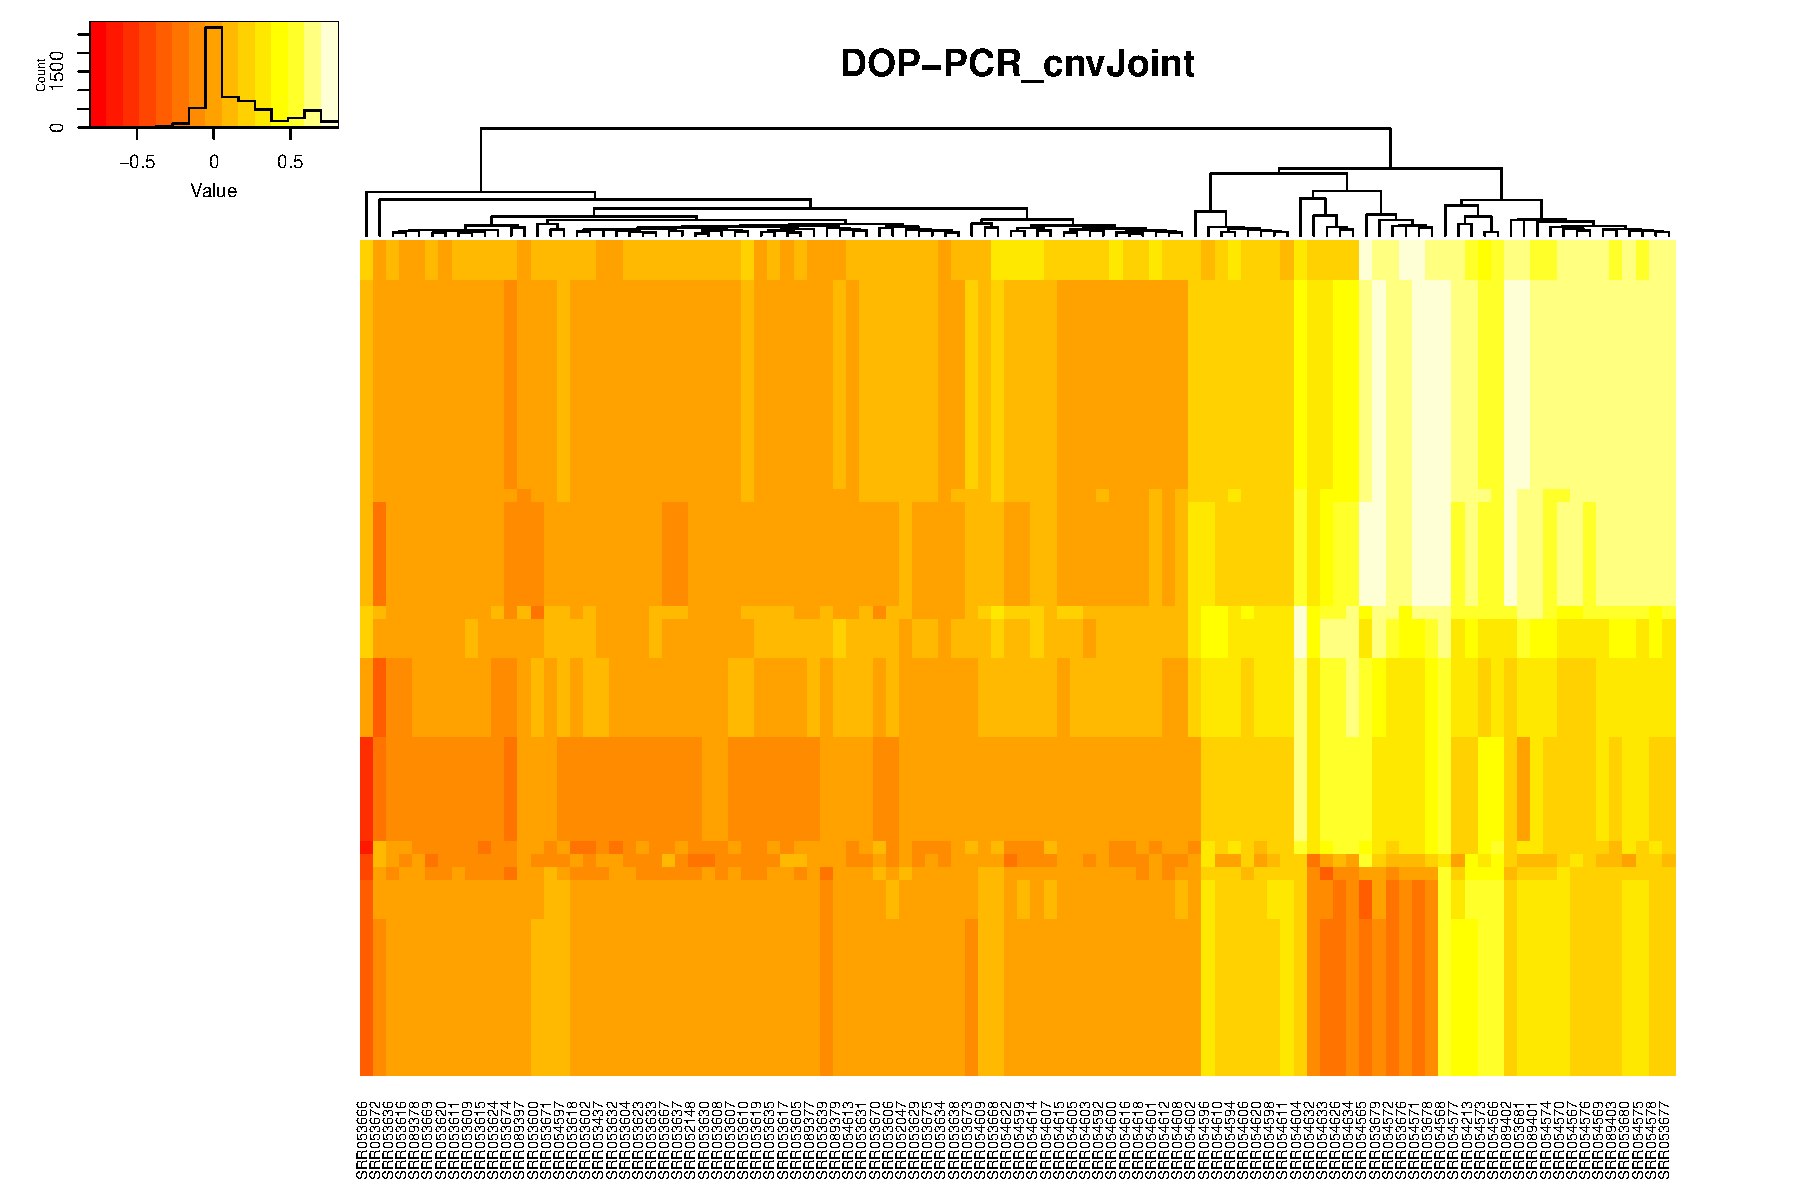
\includegraphics[width=0.49\textwidth]{poly_cnvJoint_theta_heat.pdf}\\
\includegraphics[width=0.49\textwidth]{lung_MBAmethyl_theta_heat.pdf}
\includegraphics[width=0.49\textwidth]{lung_cnvJoint_theta_heat.pdf}
    \rule{\textwidth}{1pt}
\caption{\label{thetaheatmap}\textit{
\textbf{Comparison of heatmap for $\Theta$ from cnvJoint and MBAmethyl}
}}
\end{figure}

\begin{figure}[h]
\centering
\includegraphics[width=0.8\textwidth]{encode_distmat_heat.pdf}\\
\includegraphics[width=0.8\textwidth]{poly_distmat_heat.pdf}\\
\includegraphics[width=0.8\textwidth]{lung_distmat_heat.pdf}\\
\rule{\textwidth}{1pt}
\caption{\label{distmat_heat}\textit{
\textbf{Comparison of distance matrix for $\Theta$}. The cell-cell euclidean distance in terms of copy numbers is computed for the three data sets. The clusters are determined by hierarchical clustering using euclidean distance. 
}}
\end{figure}

\begin{figure}[h]
\centering
\includegraphics[width=0.45\textwidth]{intraclusters_bar.pdf}
\includegraphics[width=0.45\textwidth]{acrossclusters_bar.pdf}\\
\caption{\label{diff_bar}
\textbf{Difference in intra-cluster and cross-cluster distance}\\
The bar graph shows that in most cases, average intra-cluster distance is smaller for cnvJoint, suggesting more homogeneity is returned by our new approach. In contrast, when average distance is computed across different clusters, e.g. between normal cells versus tumor cells, cnvJoint returned higher average distance for most cases, suggesting clearer distinction between the cell types. 
}
\end{figure}

\begin{figure}[h]
\centering
\includegraphics[width=0.8\textwidth]{dist_xi.png}
\caption{\label{dist_xi}
\textbf{Distribution of $\xi$}\\The values of $\xi$ values for the three data types. This essentially measures the effectiveness of our new method compared to MBAmethyl. Due to the nature of the data, the individual shifts have small effects on Ginkgo data sets that have been sufficiently cleaned. 
}
\end{figure}

\bibliographystyle{plain}
\bibliography{cite}


\end{document}







